\title{NNPDF}
\author[Rosalyn Pearson]{}
\institute{University of Edinburgh}
\date{PDF4LHC}

\begin{frame}{Extra: Nuclear and deuteron observables}
\footnotesize{Deuteron (top) and heavy nuclear (bottom) }
  \begin{figure}
    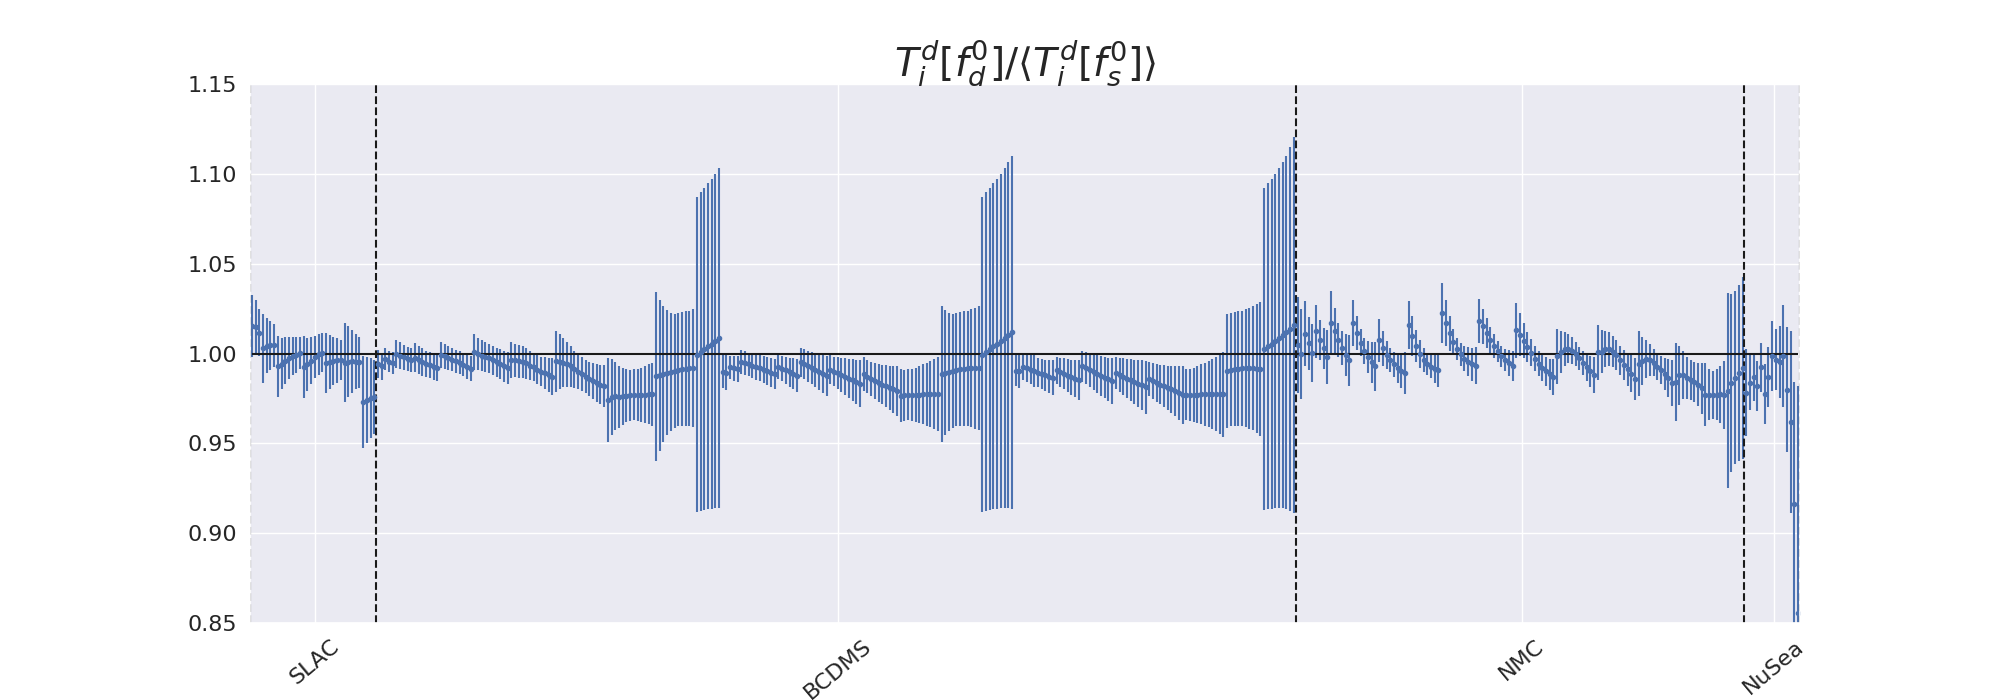
\includegraphics[width=90mm, trim={30mm, 0, 30mm, 0}]{nuclear_uncs/obsdeut.png}
    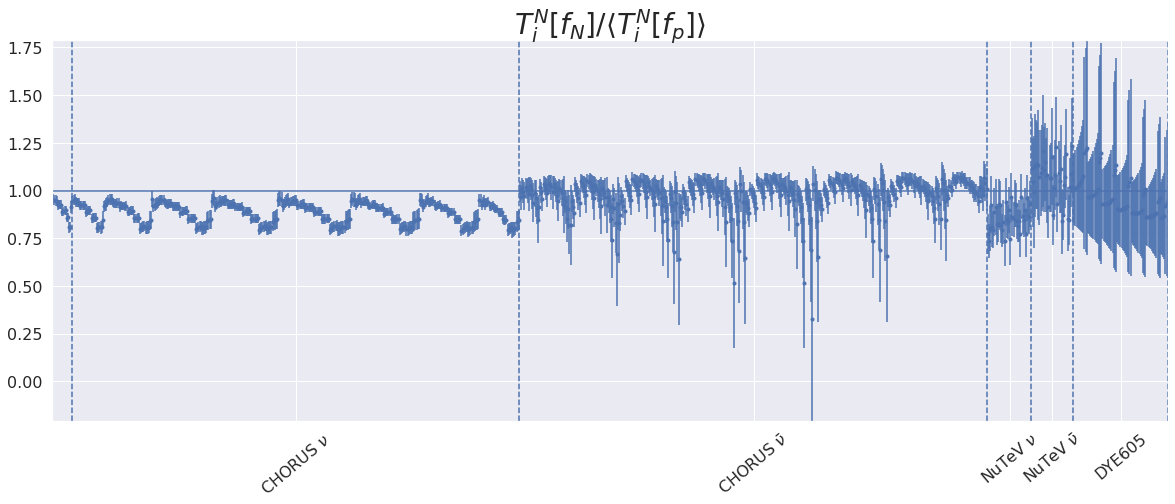
\includegraphics[width=85mm]{nuclear_uncs/obsnuc.png}
  \end{figure}
\end{frame}

\begin{frame}{Extra: deuteron uncertainties}

\begin{block}{Deuteron data}
{\bf Deuteron only} $F_2^d$: SLAC, BCDMS  $\to T_i^d[f_d]$
\newline
{\bf Mixed} $F_2^d/F_2^p$ \& $\sigma_{pd}^{DY}/\sigma_{pp}^{DY}$: NMC, DYE866/NuSea  $ \to T_i^d[f_d, f_p]$
\end{block}
Standard is to use isoscalar PDFs in place of deuteron: $f_s \equiv \frac{1}{2}(f_p + f_d)$
Now 
\begin{equation}
\Delta_i^{(k)} = \begin{cases}
T_i^d[f_d^{(k)}] - T_i^d[f_s^{(0)}] & i \in \text{deuteron only}\\
T_i^d[f_d^{(k)}, f_p^{(0)}] - T_i^d[f_s^{(0)}, f_p^{(0)}] & i \in \text{mixed}
\end{cases}
\end{equation}
\end{frame}

\begin{frame}{Extra: heavy nuclear uncertainties}

\begin{block}{Heavy nuclear data $T_i^N[f_N]$}
{\bf Cu}: DYE605,  $N=64$
\newline
{\bf Fe}: NuTeV (\& EMC), $N=56$
\newline
{\bf Pb}: CHORUS, $N=208$
\end{block}
\begin{equation}
\Delta_i^{(k)} = T_i^{N}[f_{N}^{(k)}] - T_i^{N}[f_{p}]
\end{equation}
Where 
\begin{equation}
\begin{split}
    T_i^N[f_N] = \frac{1}{A} (ZT_i[f_{p/N} + (A-Z)T_i[f_{n/N}] \\
    T_i^N[f_p] = \frac{1}{A} (ZT_i[f_p] +  (A-Z)T_i[f_n]
\end{split}
\end{equation}
\end{frame}
\begin{frame}{Extra: Correlation matrix}
  \begin{figure}
  \centering
    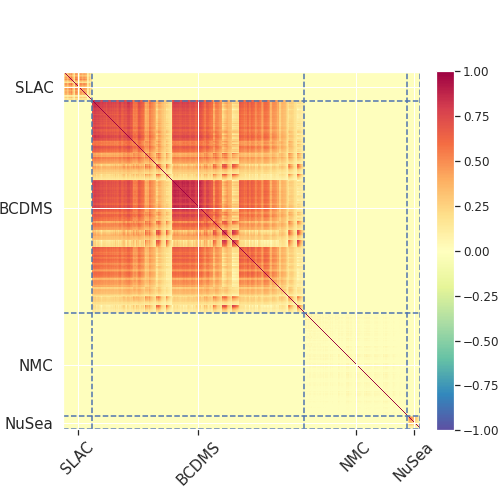
\includegraphics[width=40mm]{nuclear_uncs/covexpdeut.png}
    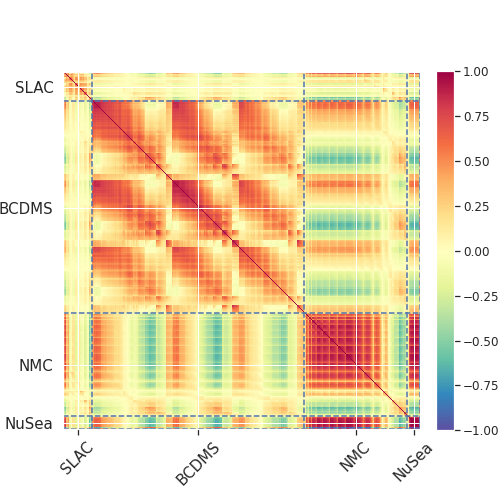
\includegraphics[width=40mm]{nuclear_uncs/covtotdeut.png}
    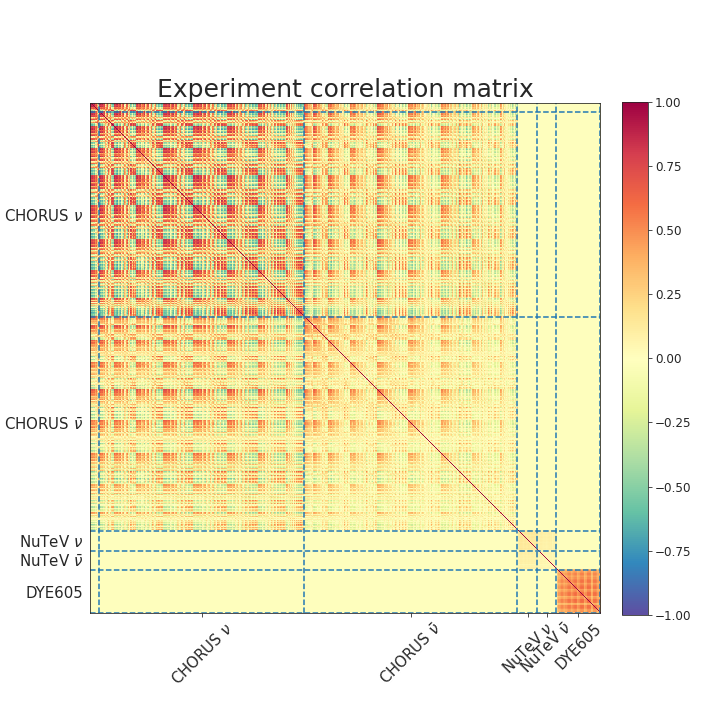
\includegraphics[width=40mm]{nuclear_uncs/covexpnuc.png}
    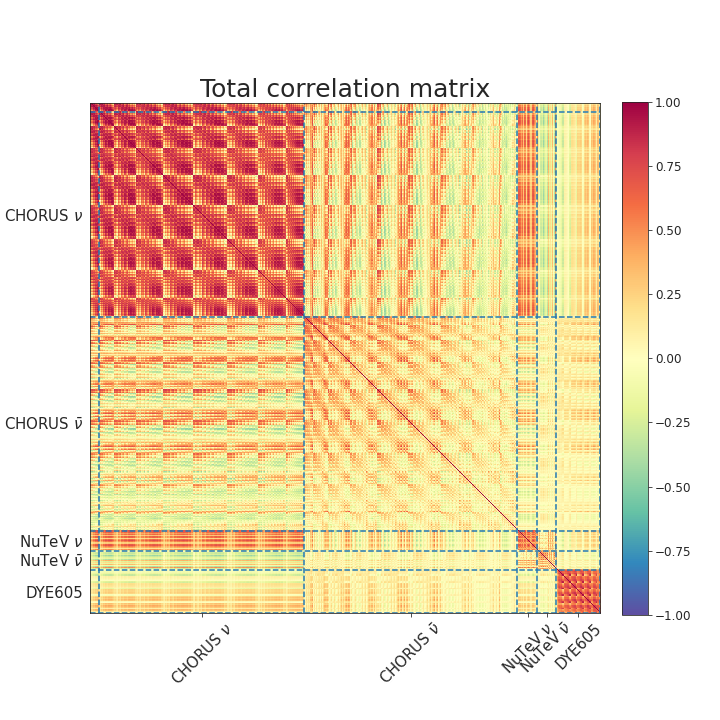
\includegraphics[width=40mm]{nuclear_uncs/covtotnuc.png}
  \end{figure}
  \end{frame}
\begin{frame}{Extra: Nuclear correction}
\begin{itemize}
\item Can also ``shift" the observables $T_i^{(N/d)}[f_(p/s)^{(0)}] \to T_i^{(N/d)}[f_{(N/d)}^{(0)}]$
\item Uncertainty is correspondingly reduced
\end{itemize}
  \begin{figure}
    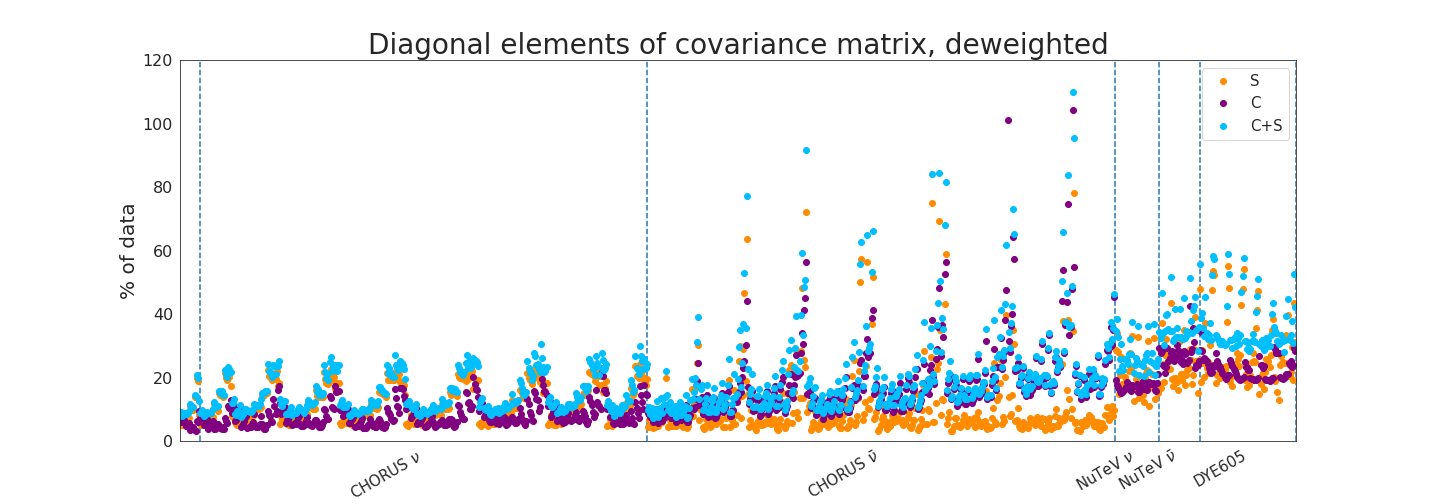
\includegraphics[width=85mm]{nuclear_uncs/diagnuc_title.png}
    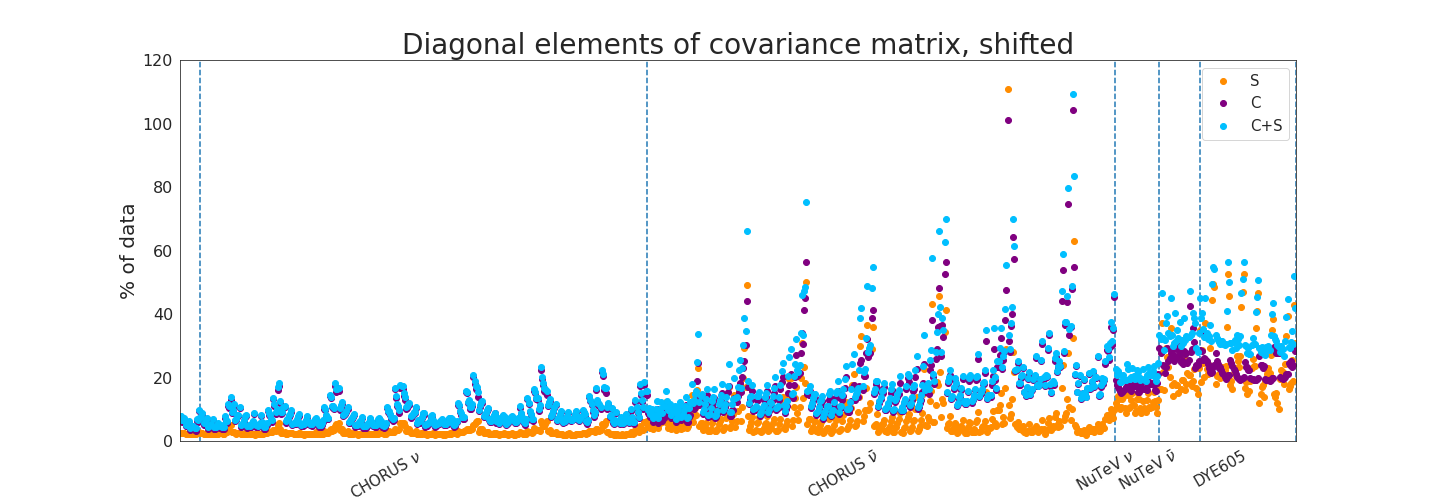
\includegraphics[width=85mm]{nuclear_uncs/diagnucshift.png}
  \end{figure}
\end{frame}
\begin{frame}{Extra: Deuteron correction}
Comparing deuteron correction to MMHT \tiny{ \textcolor{green}{[Harland-Lang et al.: Eur. Phys. J. C 75(5), 204 (2015)]}}
  \begin{figure}
    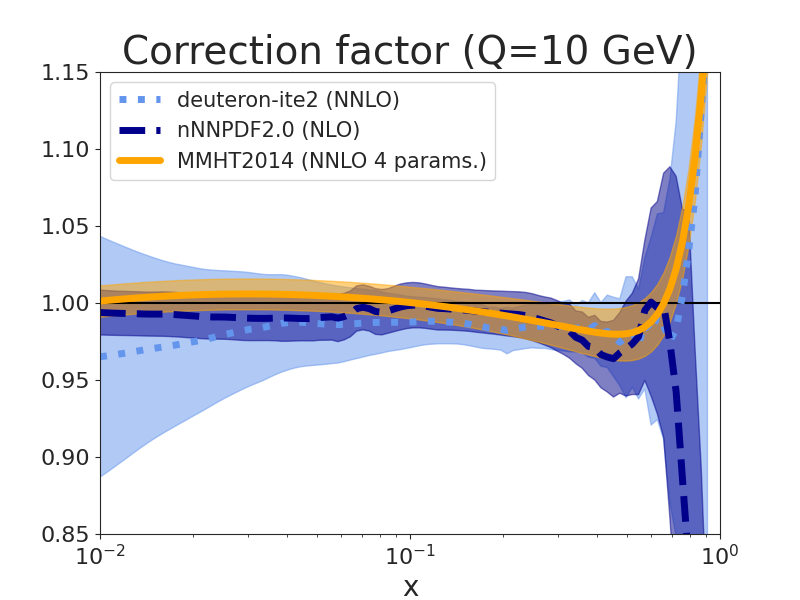
\includegraphics[width=90mm]{nuclear_uncs/corrfactor.png}
  \end{figure}
\end{frame}

\author[Zahari Kassabov]{}
\institute{University of Cambridge}
\begin{frame}{Choosing the weight}
\protect\hypertarget{choosing-the-weight}{}
\begin{itemize}
\tightlist
\item
  Not a critical setting for this kind of study.

  \begin{itemize}
  \tightlist
  \item
    Typically we see PDFs bending and/or other datasets being poorly
    fitted.
  \end{itemize}
\item
  Rule of thumb: Have the dataset contributed roughly as much to the
  total error function as all the of the data (assuming
  \(\chi^2\)/ndat=1) \[
  w = \text{total ndat}/\text{dataset ndat}
  \] e.g.~DO e ASY has 11 points and we have 4524 in total, so we set a
  weight of 411.

\end{itemize}
\end{frame}
